% ----- formatovani dokumentu -----------------------------------------------
\documentclass[12pt,a4paper,titlepage,final]{report}
\usepackage[utf8]{inputenc}
\usepackage[T1, IL2]{fontenc}
\usepackage{graphicx}
\usepackage{epstopdf}
\usepackage[margin=2cm]{caption}
\usepackage[top=3cm, left=2cm, right=2cm, text={17cm, 24cm}, ignorefoot]{geometry}
\usepackage{color}
\usepackage{url}
\usepackage{setspace}
\singlespacing
\usepackage[square, numbers]{natbib} 
\usepackage{float}
\pagestyle{plain}
\pagenumbering{arabic}
\setcounter{page}{1}
\setcounter{secnumdepth}{-1}
\setlength{\parindent}{1cm}	
\usepackage{natbib}
\usepackage{amsmath}
\usepackage{tocloft}
\usepackage{esvect}
\usepackage{amssymb}
\usepackage{gensymb}
\usepackage{subcaption}
\usepackage[algoruled,boxed,lined,longend]{algorithm2e}


\DeclareMathOperator{\dis}{d}

  \newenvironment{czechalgorithm}[1][htb]
  {\renewcommand{\algorithmcfname}{Algoritmus}% Update algorithm name
   \begin{algorithm}[#1]%
  }{\end{algorithm}}

% ----- vyberte jazyk -------------------------------------------------------
\usepackage[english,czech]{babel}
%\usepackage[english]{babel}

% ----- dopiste titulky -----------------------------------------------------
\newcommand\Course{Biometrické systémy}
\newcommand\WorkTitle{Určení natočení hlavy na základě antropometrických bodů}
\newcommand\AuthorA{Petr Flajšingr}
\newcommand\AuthorAEmail{xflajs00@stud.fit.vutbr.cz}
\newcommand\AuthorB{Igor Frank}
\newcommand\AuthorBEmail{xfrank12@stud.fit.vutbr.cz}
\newcommand\Faculty{Fakulta Informačních Technologií}
\newcommand\School{Vysoké Učení Technické v Brně}

\usepackage[
pdftitle={\WorkTitle},
pdfauthor={\AuthorA}
bookmarks=true,
colorlinks=true,
breaklinks=true,
urlcolor=blue,
citecolor=blue,
linkcolor=blue,
unicode=true,
]
{hyperref}


% ----- titulni strana ------------------------------------------------------

\begin{document}
	\begin{titlepage}
	\begin{center}
		
\includegraphics[height=5cm]{images/logo.eps}
	\end{center}
	\vfill
	\begin{center}
		\begin{Large}
			\Course\\
		\end{Large}
		\bigskip
		\begin{Huge}
			\WorkTitle\\
		\end{Huge}
	\end{center}
	\vfill
	\begin{center}
		\begin{large}
			\today
		\end{large}
	\end{center}
	\vfill
	\begin{flushleft}
		\begin{large}
			\begin{tabular}{lll}
				Autoři: & \AuthorA, & \url{\AuthorAEmail} \\
				& \AuthorB, & \url{\AuthorBEmail} \\
				& \Faculty \\
				& \School \\
			\end{tabular}
		\end{large}
	\end{flushleft}
\end{titlepage}		

\section{Úvod}
Tato technická zpráva popisuje 3 metody pro odhad natočení hlavy ve třech stupních volnosti (yaw, pitch, roll). Dále jsou zde popsány experimenty, úspěšnost detekce a také rychlost výpočtu všech metod. Zpráva také obsahuje informace o použitých technologiích a jejich případných omezení.

\section{Detekce klíčových bodů}
Pro nalezení obličeje na vstupním snímku je využita knihovna dlib\footnote{\url{http://dlib.net/}}, specificky její "frontal face detector". Pro detekci obličeje je tedy využito histogramu orientovaných gradientů (HOG) v kombinaci s metodou podpůrných vektorů (SVM).

Jak název napovídá, není tato metoda schopna detekovat obličej, který je příliš natočený. Vzhledem k našim řešením tohle ale není velkým problémem, jelikož k výpočtu využíváme oblastí, které se nachází na okraji obličeje. Jediným výraznějším nedostatkem je neschopnost detekovat obličej natočený podle Z osy (roll) o více než cca 30\degree.

K detekci klíčových bodů obličeje je opět využita knihovna dlib. 

\begin{figure}[H]
    \centering
    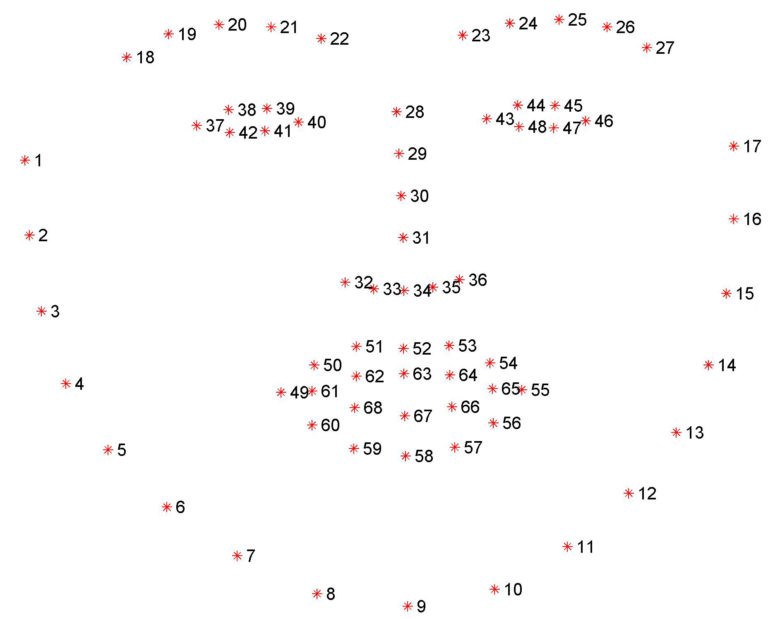
\includegraphics[scale=0.35]{images/detected_landmarks.jpeg}
    \caption{Klíčové body detekované pomocí dlib. Zdroj: \url{https://ibug.doc.ic.ac.uk/resources/300-W/}}
    \label{fig:dlib_key_points}
\end{figure}

Tyto body korespondují bodům v \cite{antro_points}, díky čemuž můžeme využít vztahů popsaných v této publikaci.

\section{Odhad natočení hlavy}
Estimace natočení hlavy může být řešena různými způsoby. Mezi populární metody patří především PnP, která je zmíněna dále. Samozřejmostí je také využití strojového učení pro odhad, jelikož se ale tyto metody nezabývají přímo geometrií obličeje a vztahy mezi klíčovými body, nejsou v našem řešení využity.

Metody popsané v této sekci odhadují natočení hlavy ve třech stupních volnosti -- yaw, pitch a roll. 

\begin{figure}[H]
    \centering
    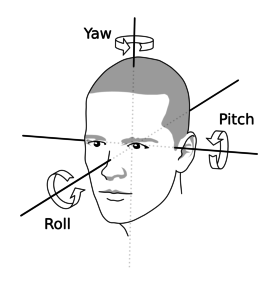
\includegraphics[scale=2]{images/yaw_pitch_roll.png}
    \caption{3 stupně volnosti natočení hlavy. Zdroj: \url{https://www.researchgate.net/publication/305684696_On_the_rhythm_of_head_movements_in_Finnish_and_Swedish_Sign_Language_sentences}}
    \label{fig:yaw_pitch_roll}
\end{figure}

\subsection{Metoda 1.: PnP}
Metoda PnP byla převážně použita pro pro kontrolu ostatních metod při jejich implementaci. Jedná se o metodu, kde je hledána transformace mezi nalezenými klíčovými body ze snímku a 3D modelem obličeje. 

V implementaci byl použit zjednodušený obecný model o 6 bodech. Konkrétně se jedná o body ve vzdálenějším rohu levého a pravého oka (body 37, 46), koutky úst (body 49, 55), špička nosu (bod 31) a brada (bod 9). Pro výpočet je však potřeba znát navíc ještě optický střed kamery a ohniskovou vzdálenost. Jelikož ve většině případů jsou tyto údaje neznámé, musejí být vhodně aproximovány. 

Následně je aplikována metoda \texttt{cv2.solvePnP}, pomocí které získáme translaci a rotaci pro namapování obličeje na 3D model. Metoda byla použita s využitím Levenberg–Marquardtova algoritmu poskytnutém knihovnou openCV. Algoritmus je numerickou metodou snažící se iterativně co nejvíce přiblížit lokálnímu minimu přičítáním vypočtených hodnot k počátečnímu odhadu.

\subsection{Metoda 2.: Tracking}
Na rozdíl od metody uvedené v předchozí sekci odhad natočení hlavy pomocí tracking (sledování pohybu) vyžaduje více snímků pro svoji funkčnost. Není tedy možné odhadnout úhly na základě jednoho snímku. Na místo toho je využit první snímek jako inicializační -- předpokládá se, že první snímek má tedy všechny úhly nulové. Vhodným rozšířením by byla inicializace za pomocí jedné z ostatních metod. Metoda byla implementována na základě \cite{est_for_mobile}.

Hlavním cílem této metody je především vysoká rychlost, jak můžete vidět v sekci vyhodnocení rychlosti.

\subsubsection{Roll}
Roll je odhadnut jednoduchým způsobem -- skrz body na okraji očí (obrázek \ref{fig:roll}) je proložena přímka. Na základě jejího úhlu vůči x-ové ose je přímo spočten úhel roll. Střed otáčení je pro tento výpočet místo spojení páteře a lebky. Vzorec pro výpočet tohoto úhlu je rovnice \ref{eq:roll}.

\begin{equation}\label{eq:roll}
roll=\arctan{\frac{p_x^{right\_eye\_corner} - p_x^{left\_eye\_corner}}{p_y^{right\_eye\_corner} - p_y^{left\_eye\_corner}}}
\end{equation}

\begin{figure}[H]
    \centering
    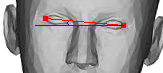
\includegraphics[scale=1.5]{images/roll.jpg}
    \caption{Ilustrace výpočtu roll}
    \label{fig:roll}
\end{figure}

\subsubsection{Yaw a pitch}
Yaw a pitch jsou počítány za pomocí rozdílu polohy špičky nosu proti předcházejícímu snímku. Abychom mohli tento rozdíl přepočítat na úhel, je nutné zvolit střed otáčení. Jako střed jsme zvolili střed hlavy -- tedy bod nacházející se stejnou vzdáleností mezi obličejem a zadní stranou hlavy. Tuto vzdálenost lze vypočíst za pomocí vztahu \ref{eq:mid_dist}, kde \textit{ratio} je poměr vzdálenosti očí a průměrné hloubky hlavy \cite[str.~73]{antro_points}.

\begin{equation}\label{eq:mid_dist}
r=\lVert \mathbf{p^{right\_eye\_corner} - p^{left\_eye\_corner}} \rVert \cdot ratio / 2
\end{equation}

Dále použijeme vypočtené \textit{r} jako vzdálenost ke středu otáčení a rozdíl na jednotlivých osách mezi snímky jako rozdíl pro pohyb na kružnici. Vypočtený úhel je v každém snímku přičten k výslednému úhlu. 

\begin{equation}\label{eq:x_delta}
\Delta x = p^{nose}_{x\_old} - p^{nose}_{x\_new}
\end{equation}

\begin{equation}\label{eq:tr_yaw}
yaw = yaw + \Delta x \cdot \pi \cdot 2 r \cdot modif
\end{equation}

\textit{modif} v předcházející rovnici označuje modifikátor pro opsaný úhel, který se mění na základě toho, jak velký je úhel natočení v předcházejícím kroku.

Výpočet pro pitch je stejný, ovšem pro y-ovou osu.


\subsection{Metoda 3.: Geometrie}
Výpočty použité v této metodě závisí pouze na antropometrických bodech a jejich vzájemných vztazích. Výpočty jsou založeny na \cite{murphy-chutorian_trivedi_2009}.
\subsubsection{Roll}
Pro tuto metodu je roll vypočítán naprosto stejným způsobem jako pro metodu předcházející. Jedná se tedy o úhel přímky procházející okraji očí oproti x-ové ose.

\subsubsection{Yaw}
Princip výpočtu yaw je následující. Můžeme předpokládat, že úhel lze určit odchylkou nějakého středového bodu obličeje od osy y. Jako tento středový bod jsme zvolili bod nacházející se pod nosem. Jako další pomocné body jsme zvolili ty, které se nacházejí na okraji obličeje. 

\begin{figure}[H]
    \centering
    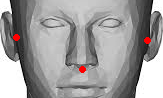
\includegraphics[scale=1.5]{images/yaw_points.jpg}
    \caption{Body použité pro výpočet yaw}
    \label{fig:roll}
\end{figure}

Prvním krokem výpočtu je proložení zmíněných bodů přímkou. Proto spočteme nejdříve údaje přímky za pomocí rovnice \ref{eq:slope} pro směrnici(\textit{k}) a rovnice \ref{eq:q} pro úsek(\textit{q}).

\begin{equation}\label{eq:slope}
k = \frac{x_{p1} - x_{p2}}{y_{p1} - y_{p2}} 
\end{equation}

\begin{equation}\label{eq:q}
q = y_{p1} + k \cdot x_{p1}
\end{equation}

Následně spočteme směrnici přímky procházející bodem pod nosem, která je kolmá k přímce procházející mezi okraji obličeje. Směrnici lze spočítat pomocí rovnice \ref{eq:inv_slope}. Pro výpočet úseku opět využijeme rovnice \ref{eq:q} s bodem pod nosem.

\begin{equation}\label{eq:inv_slope}
k_2 = -\frac{1}{k}
\end{equation}

Dalším krokem je nalezení průsečíku vypočtených přímek, čímž umístíme centrální bod na přímku mezi okraji obličeje. Toho lze dosáhnout pomocí rovnic \ref{eq:line_inters_x} a \ref{eq:line_inters_y}.

\begin{equation}\label{eq:line_inters_x}
x_i = \frac{q_2 - q}{k - k_2}
\end{equation}

\begin{equation}\label{eq:line_inters_y}
y_i = k \cdot x_i + q
\end{equation}

Posledním krokem je výpočet samotného úhlu. Nejdříve spočteme pozici středu hlavy. Tu lze spočítat jako bod nacházející se mezi body na okraji obličeje -- rovnice \ref{eq:mid_head}. 

\begin{equation}\label{eq:mid_head}
\vec{v}_{mid} = \frac{\vec{v}_{p1} + \vec{v}_{p2}}{2}
\end{equation}

Dále potřebujeme znát vzdálenost od nosu do středu hlavy. Pro tento výpočet můžeme využít poměru vzdálenosti okrajů obličeje a "hloubky" hlavy, čímž získáme konstantu $a = 0.7$.
 
\begin{equation}\label{eq:geom_yaw}
yaw = \arcsin{(\frac{\lVert \mathbf{p_i - p_{mid}} \rVert}{\lVert \mathbf{p_1 - p_2} \rVert} \cdot a)}
\end{equation}

\subsubsection{Pitch}
Jak je vidět na obrázku \ref{fig:pitch} pitch lze spočítat podle poměru vzdálenosti špičky nosu od přímky mezi očima a přímky procházející ústy.

\begin{figure}[H]
    \centering
    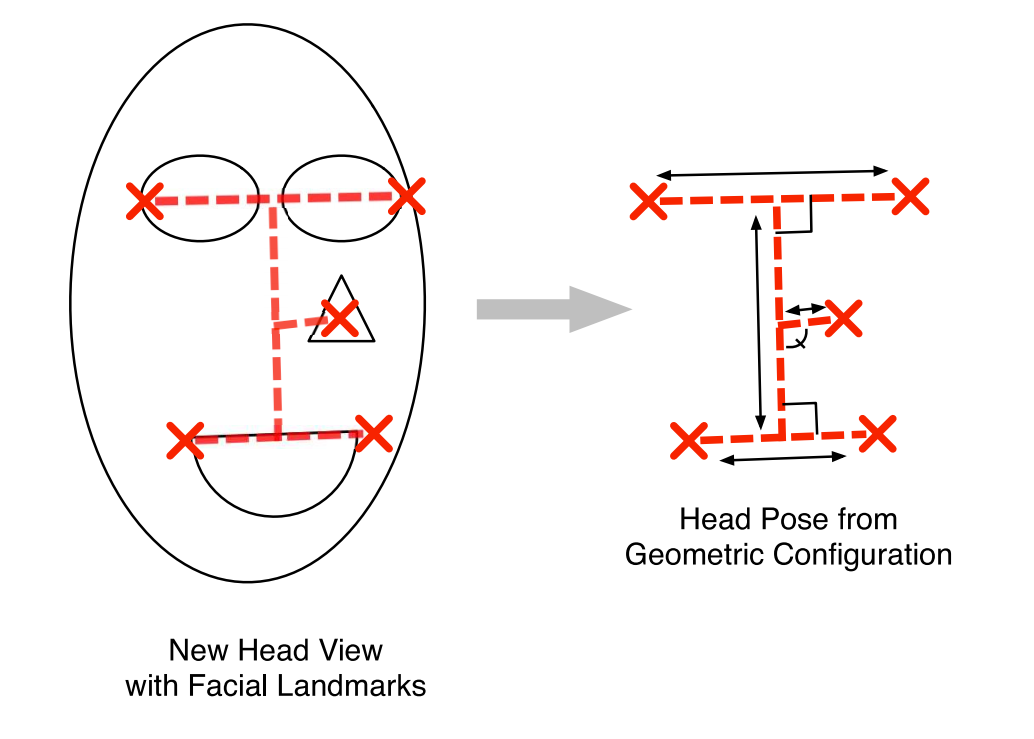
\includegraphics[scale=0.3]{images/pitch_geom.png}
    \caption{Body použité pro výpočet pitch. Zdroj: \cite{murphy-chutorian_trivedi_2009}}
    \label{fig:pitch}
\end{figure}

Nejdříve je tedy nutné spočítat bod nacházející se mezi očima. K tomu využijeme rovnice \ref{eq:mid_head}. Obdobně pro ústa. 

Další potřebnou hodnotou je pozice průsečíku přímky procházející mezi výše vypočtenými body. Proto spočteme parametry této přímky pomocí rovnic \ref{eq:slope} a \ref{eq:q}. Pro směrnici kolmice využijeme rovnice \ref{eq:inv_slope} a pro parametr $q$ použijeme rovnici \ref{eq:q} s dosazením pozice bodu špičky nosu.

Spočtené hodnoty nám umožňují určit poměrnou vzdálenost špičky nosu od bodu mezi očima resp. ústy. To odpovídá poměrné vzdálenosti hran trojúhelníku procházející zmíněnými body -- rovnice \ref{eq:ratio}. Rotace tohoto trojúhelníku určuje pitch. Proto platí rovnice \ref{eq:pitch_angles} kde $l_{nose}$ je hloubka nosu, $l_{mouth}$ je vzdálenost nosu a úst,  $l_{eyes\_mouth}$ je vzdálenost bodů mezi očima a ústy a $\alpha$ je pitch.

\begin{equation}\label{eq:ratio}
Q = \frac{y_{mouth} - y_{nose}}{y_{eyes} - y_{mouth}}
\end{equation}

\begin{equation}\label{eq:pitch_angles}
Q = \frac{l_{nose}\sin{\alpha} + l_{mouth}\cos{\alpha}}{l_{eyes\_mouth}\cos{\alpha}}
\end{equation}

Jelikož naším cílem je zjistit úhel pitch ($\alpha$), musíme rovnici upravit -- rovnice \ref{eq:pitch_calc}. Po dosazení hodnot odvozených z tabulek antropometrických měření můžeme vypočítat \textit{pitch}.

\begin{equation}\label{eq:pitch_calc}
\alpha = \arctan{\frac{Q - \frac{l_{mouth}}{l_{eyes\_mouth}}}{\frac{l_{nose}}{l_{eyes\_mouth}}}}
\end{equation}

\section{Implementace}
\subsection{Použité technologie}
Všechny představené metody byly implementovány v jazyce Python3\footnote{\url{https://www.python.org/}}. Pro práci s vektory/maticemi je využita knihovna numpy\footnote{\url{https://numpy.org/}}. Pro samotnou práci s obrazem je použita knihovna OpenCV\footnote{\url{https://opencv.org/}} a dlib. K vygenerování grafů pro vyhodnocení byla použita knihovna plotly\footnote{\url{https://plot.ly}}.

Pro vývoj jsme využili IDE PyCharm\footnote{\url{https://www.jetbrains.com/pycharm/}} a verzovacího systému git. Repository je možné najít na adrese \url{https://github.com/PetrFlajsingr/BIO-head-pose-estimation}.
\subsection{Použití programu}
Použití je uvedeno v souboru \texttt{README.md} nacházející se ve složce skriptu, případně je lze zjistit pomocí přepínače \texttt{-h}.

\section{Experimenty a vyhodnocení}
Vyhodnocení bylo provedeno nad datasetem Gaze Interaction for Everybody (dále jen GI4E\footnote{\url{http://www.unavarra.es/gi4e/databases}}), který veřejně poskytuje Public University of Navarra. Poskytované datasety jsou ve formě videí s přiloženými údaji o natočení osoby v každém snímku videa. Níže jsou uváděny grafy reprezentující červenou křivkou námi vyhodnocené úhly natočení a modrou křivkou údaje poskytnuté v datasetu. Všechny poskytnuté grafy se vztahují k totožnému videu, ve kterém jsou zastoupeny postupně všechny úhly natočení.
\subsection{Metoda 1.: PnP}
Metoda PnP přesně kopíruje křivku očekávaných hodnot, s tím že rozmezí chyby je řádově v jednotkách stupňů. Tím pádem bychom mohli tuto metodu zařadit mezi přesnější metody, nicméně je patrná skoková změna i ve větších hodnotách mezi jednotlivými snímky vytvářející nehladký průběh grafu s občasnými špičkami.

\begin{figure}[H]
  \centering
  \captionsetup{justification=centering}
  \begin{subfigure}[b]{0.32\textwidth}
    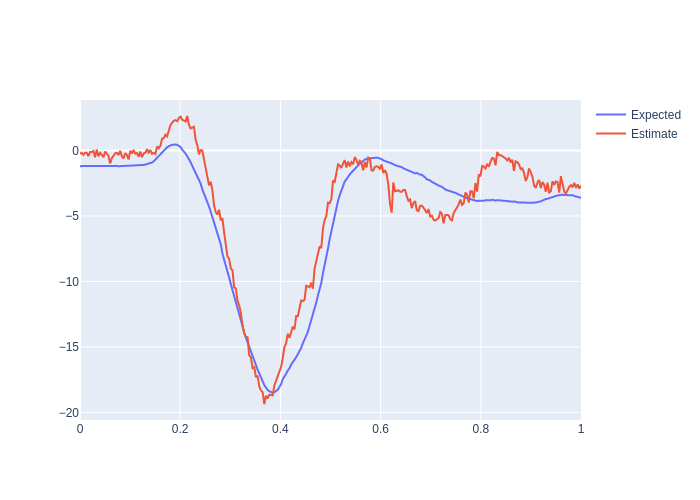
\includegraphics[width=\textwidth]{images/evaluation/3D_model_roll_user_01_video_07.png}
   \caption{Roll}
    \label{fig:pnp_roll}
  \end{subfigure}
  \hfill
  \begin{subfigure}[b]{0.32\textwidth}
    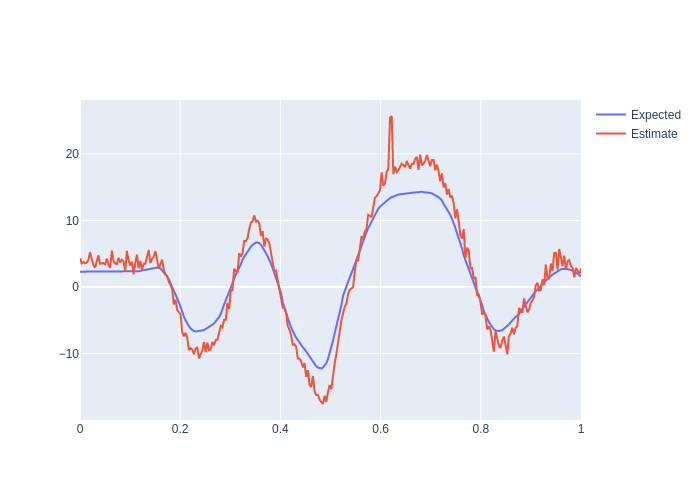
\includegraphics[width=\textwidth]{images/evaluation/3D_model_yaw_user_01_video_07.png}
   \caption{Yaw}
    \label{fig:pnp_yaw}
  \end{subfigure}
  \hfill
    \begin{subfigure}[b]{0.32\textwidth}
    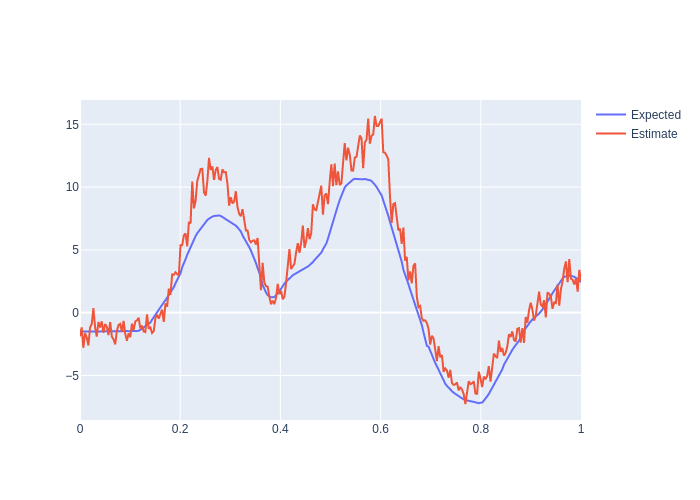
\includegraphics[width=\textwidth]{images/evaluation/3D_model_pitch_user_01_video_07.png}
   \caption{Pitch}
    \label{fig:pnp_pitch}
  \end{subfigure}
  \caption{Srovnání průběhu pro metodu PnP}
  \label{fig:pnp_graphs}
\end{figure}

\subsection{Metoda 2.: Tracking}
Výpočet úhlu roll je zde přesnější než při metodě PnP, nicméně u úhlů yaw a pitch metoda velmi zaostává. Přestože průběh grafu metody trakcing je velmi hladký a opět do jisté míry kopíruje křivku představující pravdivé hodnoty, u úhlů pitch a yaw jsou vypočítané hodnoty velmi odlišné.

\begin{figure}[H]
  \centering
  \captionsetup{justification=centering}
  \begin{subfigure}[b]{0.32\textwidth}
    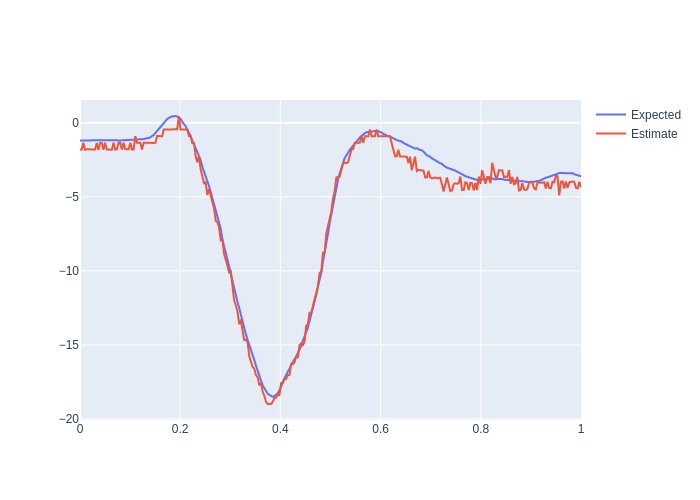
\includegraphics[width=\textwidth]{images/evaluation/tracking_roll_user_01_video_07.png}
   \caption{Roll}
    \label{fig:track_roll}
  \end{subfigure}
  \hfill
  \begin{subfigure}[b]{0.32\textwidth}
    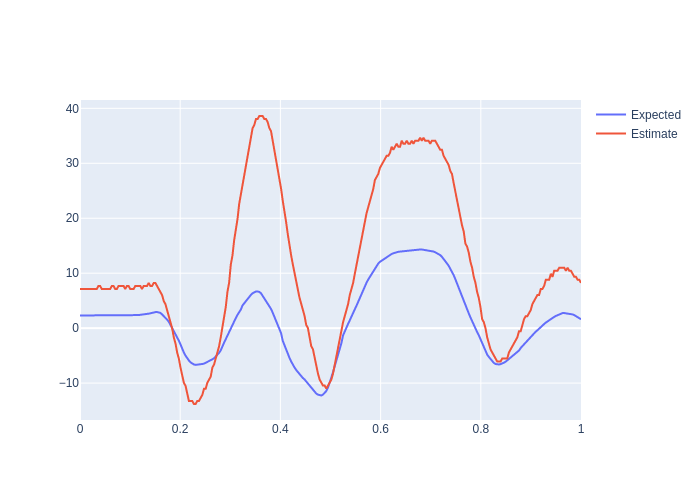
\includegraphics[width=\textwidth]{images/evaluation/tracking_yaw_user_01_video_07.png}
   \caption{Yaw}
    \label{fig:track_yaw}
  \end{subfigure}
  \hfill
    \begin{subfigure}[b]{0.32\textwidth}
    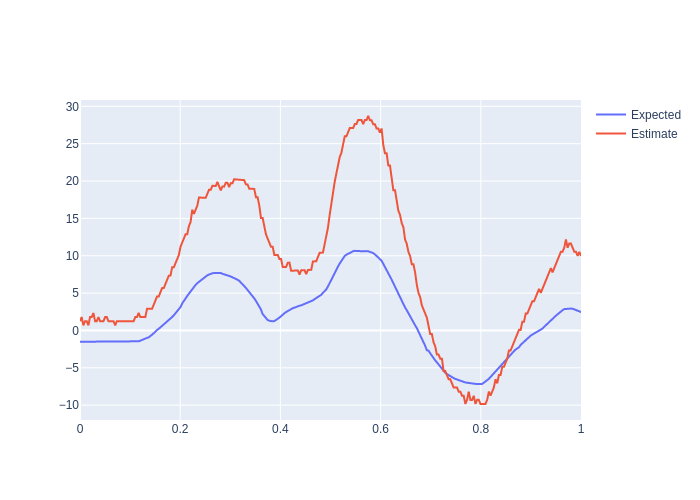
\includegraphics[width=\textwidth]{images/evaluation/tracking_pitch_user_01_video_07.png}
   \caption{Pitch}
    \label{fig:track_pitch}
  \end{subfigure}
  \caption{Srovnání průběhu pro metodu tracking}
  \label{fig:track_graphs}
\end{figure}

\subsection{Metoda 3.: Geometrie}
Metoda využivající vzathy antropometrických bodů vykazuje na grafu přibližně podobné výsledky jako metoda PnP, s tím rozdílem, že má velmi přesný roll úhel stejně jako metoda tracking. Nicméně i zde dostáváme často "zubovitý" tvar grafu.

\begin{figure}[H]
  \centering
  \captionsetup{justification=centering}
  \begin{subfigure}[b]{0.32\textwidth}
    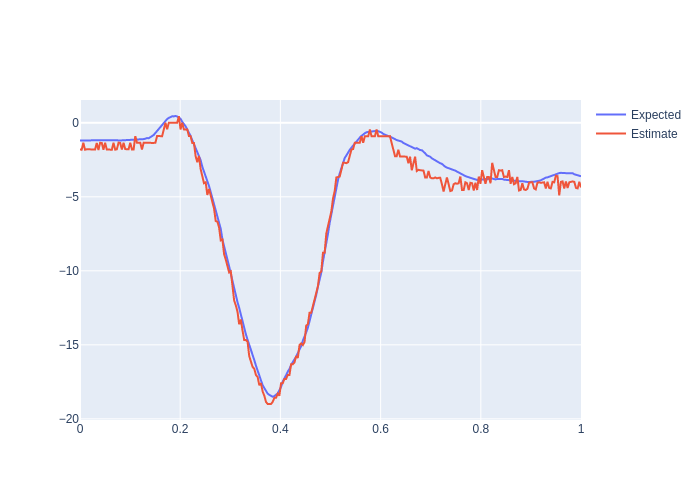
\includegraphics[width=\textwidth]{images/evaluation/geometry_roll_user_01_video_07.png}
   \caption{Roll}
    \label{fig:geo_roll}
  \end{subfigure}
  \begin{subfigure}[b]{0.32\textwidth}
    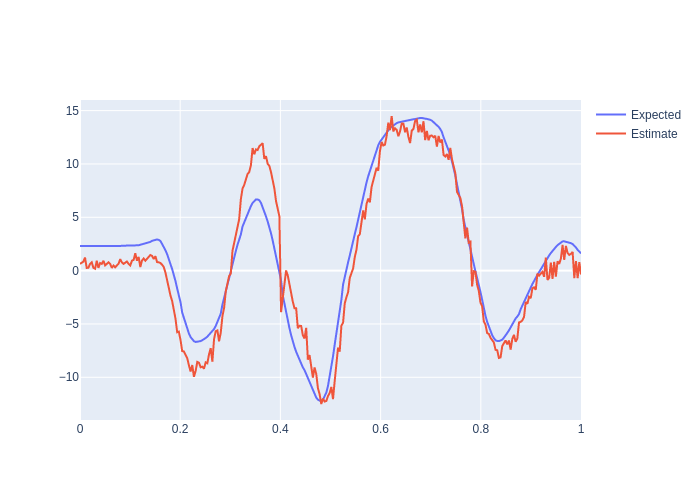
\includegraphics[width=\textwidth]{images/evaluation/geometry_yaw_user_01_video_07.png}
   \caption{Yaw}
    \label{fig:geo_yaw}
  \end{subfigure}
    \begin{subfigure}[b]{0.32\textwidth}
    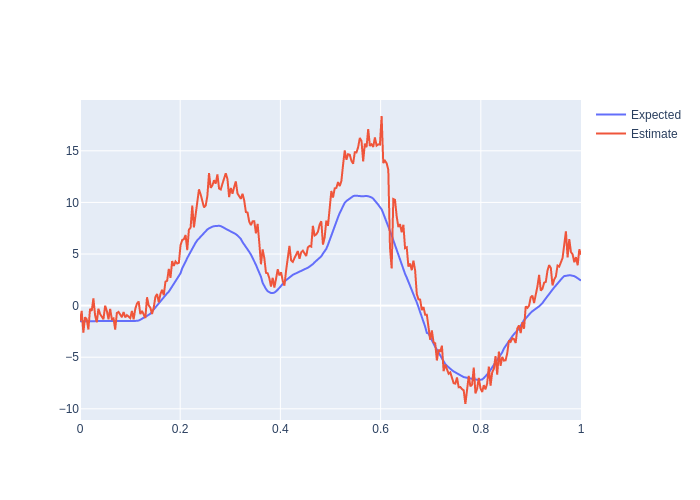
\includegraphics[width=\textwidth]{images/evaluation/geometry_pitch_user_01_video_07.png}
   \caption{Pitch}
    \label{fig:geo_pitch}
  \end{subfigure}
  \caption{Srovnání průběhu pro metodu využívající geometrii}
  \label{fig:geo_graphs}
\end{figure}

\subsection{Srovnání metod}
Při využití metody na základě PnP a geometrie dostáváme nejpřesnější výsledky, nicméně i zde jsou pozorovány silné odchylky. Tyto odchylky závisí na přesnosti výpočtu klíčových bodů obličeje a v případě metody PnP vznikají i použitím obecného modelu obličeje daného pouze několika body, a aproximací vlastností kamery. 

Chyby u geometrické metody pak navíc mohou vznikat z předpokladu dokonalého a symetrického obličeje. U metody sledování bodů nastává problém, pokud dochází k pohybu hlavy bez rotace. Výše popsaná metoda pak pohyb chybně vyhodnotí jako rotaci a dochází k odchýlení od pravdivých hodnot. Přes zmíněné omezení jde však o velice rychlou metodu vhodnou pro mobilní zařízení. 

Níže jsou uvedeny údaje průměrné chyby a směrodatné odchylky vypočítané vůči databázi GI4E nad několika z obličejů. Výsledné hodnoty jsou pro přehlednost zaokrouhleny.

\begin{table}[h]
\centering
\begin{tabular}{|l|l|l|l|}
\hline
\textit{Metoda PnP}                & \textbf{Roll[\degree]} & \textbf{Yaw[\degree]} & \textbf{Pitch[\degree]} \\ \hline
\textbf{Průměrná absolutní chyba}  & 1.87944819  & 3.846113639 & 4.587338469    \\ \hline
\textbf{Průměrná směrodatná odchylka chyby} & 4.914020841 & 6.139181454 & 4.162728145     \\ \hline
\end{tabular}
\caption{Chyby metody PnP}
\label{tab:pnp_err}
\end{table}

\begin{table}[h]
\centering
\begin{tabular}{|l|l|l|l|}
\hline
\textit{Metoda tracking}                & \textbf{Roll[\degree]} & \textbf{Yaw[\degree]} & \textbf{Pitch[\degree]} \\ \hline
\textbf{Průměrná absolutní chyba}  & 0.586350138 & 8.203542315 & 4.341512761    \\ \hline
\textbf{Průměrná směrodatná odchylka chyby} & 1.184606309  & 15.071397189 & 6.313952331     \\ \hline
\end{tabular}
\caption{Chyby metody tracking}
\label{tab:track_err}
\end{table}

\begin{table}[h]
\centering
\begin{tabular}{|l|l|l|l|}
\hline
\textit{Metoda geometrie}                & \textbf{Roll[\degree]} & \textbf{Yaw[\degree]} & \textbf{Pitch[\degree]} \\ \hline
\textbf{Průměrná absolutní chyba}  & 0.582392442 & 4.834934991 & 5.987510525    \\ \hline
\textbf{Průměrná směrodatná odchylka chyby} & 1.179549572 & 4.317855862 & 3.039883609     \\ \hline
\end{tabular}
\caption{Chyby metody geometrie}
\label{tab:geo_err}
\end{table}

\section{Srovnání rychlosti}
Měření probíhalo na macOS 10.15 s CPU Intel Core i5 7360U. Hodnoty v tabulce jsou průměrem ze 100000 výpočtů. Jedná se pouze o doby výpočtu samotných metod, detekce obličejů a klíčových bodů není v měření zahrnuta.

\begin{table}[H]
\centering
\begin{tabular}{|l|r|r|}
\hline
Metoda    & \multicolumn{1}{l|}{Průměrné FPS} & Průměrná doba zpracování snímku \\ \hline
PnP       & 2367                              & 422 $\mu$s                      \\ \hline
Tracking  & 125666                            & 8 $\mu$s                        \\ \hline
Geometrie & 21776                             & 45 $\mu$s                       \\ \hline
\end{tabular}
\caption{Srovnání rychlostí použitých metod}
\label{tab:speed}
\end{table}

\section{Závěr}
Implementované metody dostačují pro přibližné určení natočení hlavy, nicméně pro přesnější výsledky by bylo nutné je metody zdokonalit, případně přijít s alternativou. 

U metody PnP by například stálo za to experimentovat s rozdílnými modely obličeje, lišící se počtem a hodnotami bodů, případně využít rozdílné algoritmy pro řešení poskytované v knihovně OpenCV. Při známých vlastnostech kamery by došlo opět k dalšímu zpřesnění. 

U výpočtu pomocí geometrie by bylo vhodné prozkoumat možnost využít přesnější geometrický modelu s použitím vícero bodů a zamyslet se a případně určitým způsobem zakomponovat rozdíly etnické, pohlaví a stáří.

\nocite{est_for_mobile}
\bibliographystyle{plain}
\begin{flushleft}
  \bibliography{references}
\end{flushleft}

\end{document}

